\documentclass{article}
\usepackage[left=2cm,right=2cm,top=2cm,bottom=2cm]{geometry}
\usepackage[utf8]{inputenc}
\usepackage[german]{babel}
\usepackage{amsmath}
\usepackage{dsfont}
\usepackage[export]{adjustbox}
\usepackage{amsthm}
\usepackage{color}
\usepackage{amsfonts}
\usepackage{amssymb}
\usepackage{wasysym}
\usepackage{makeidx}
\usepackage{graphicx}
\usepackage[colorlinks=true,urlcolor=blue,linkcolor=blue]{hyperref}
\usepackage{ziffer}
\usepackage{minted}
\usepackage{xcolor}
\usepackage{framed}
\usepackage{mdframed}
\usepackage{subfiles}
\usemintedstyle{emacs}

\definecolor{purp}{HTML}{9A72AC}
\definecolor{re}{HTML}{FC6255}
\definecolor{gre}{HTML}{83C167}
\definecolor{blu}{HTML}{58C4DD}
\definecolor{shadecolor}{rgb}{0.85,0.85,0.85}
\definecolor{bg}{rgb}{0.95,0.95,0.95}
\setlength{\parindent}{0em} 

\BeforeBeginEnvironment{minted}{\begin{mdframed}[linewidth =2 ,backgroundcolor=bg , linecolor=black, linewidth=0.5]}
\AfterEndEnvironment{minted}{\end{mdframed}}

\newtheorem{defi}{Definition}
\BeforeBeginEnvironment{defi}{\begin{mdframed}[linewidth =2 ,backgroundcolor=bg , linecolor=black, linewidth=0.5]}
\AfterEndEnvironment{defi}{\end{mdframed}}

\newcommand{\bsp}{\textbf{Beispiel}:}
%\newcommand{\task}{\textbf{Aufgabe}:}

\newcommand{\bol}[1]{\textbf{#1}}
\newcommand{\q}[1]{\glqq #1\grqq}
\newcommand{\DODO}[1]{\textbf{\textcolor{red}{DODO:}} #1 \\ \begin{center}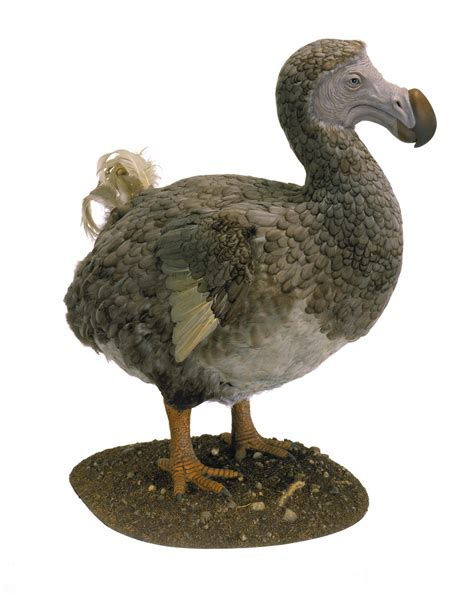
\includegraphics[scale=0.2]{../../media/dodo.jpg} \end{center}}

\newenvironment{task}[1]{
    \begin{shaded*}
    \textbf{Aufgabe #1}:
}{
    \end{shaded*}
}

\begin{document}

\subsection{Parallele Prozesse allgemein}

Neben den grundlegenden inhaltlichen Herausforderungen, die das Programmieren mit sich bringt, ist die gleichzeitige Verwendung von \textbf{Ressourcen} bei der Arbeit im Team noch eine zusätzliche Schwierigkeit. Das beginnt beispielsweise schon damit, dass in der Regel nicht zwei Entwickler an der gleichen Datei arbeiten können, wenn sie sich einfach irgendwo in einem Ordner befindet. \\
Die Beschäftigung mit solchen Problemen ist dabei so wichtig (und hat auch technische Auswirkungen), dass sich eine eigene Theorie darum aufgebaut hat. Für das Abtiur müssen die Grundlagen dieser Theorie ebenfalls verstanden werden. Für das konkrete Projekt finden sich Anmerkungen - z.B. zur Versionskontrolle und der effektiven Zusammenarbeit mit verschiedenen Tools - wie immer im Kapitel \q{Das Projekt}. Hier soll es um die theoretischen Hintergründe und Fachbegriffe gehen. \\
Als Ausgangslage stellen wir uns zwei Prozesse vor, die in irgendeiner Form in \textbf{Konkurrenz} zueinander stehen. Beispielsweise zwei Programme, die beide auf bestimmte Daten im Arbeitsspeicher zugreifen wollen. \\
Die Probleme liegen hier auf der Hand, wird der Bereich des Arbeitsspeichers von einem Program bearbeitet, während das andere ebenfalls bereits darauf zugegriffen hat, so entstehen Inkonsistenzen und Fehler. \\
\textbf{Erinnerung:} Das Problem ist bereits aus der Mittelstufe von Datenbanken bekannt, dort wurden Anomalien definiert. Im Folgenden ein Auszug aus einem Arbeitsblatt (der Text bezieht sich auf eine Tabelle Bestellung, in der Informationen zu Kunden und gekauften Artikeln vorhanden sind): \\
\q{... Es gibt jedoch noch weitere Probleme (auch Anomalien genannt), die durch Redundanzen entstehen, z.B. die UPDATE-Anomalie.\\
Wird einer oder mehrere Einträge einer Tabelle geändert, so spricht man von einem update (da der zugehörige SQL-Befehl ebenfalls UPDATE heißt!). Offensichtlich ist z.B. eine Namensänderung eines Kunden - beispielsweise durch Heirat - hier sehr problematisch, da jede einzelne seiner Bestellungen geändert werden muss, ansonsten ist die Datenbank inkonsistent. Das bedeutet, dass sie Widersprüche enthält.  \\

Möchte man etwas aus einer Tabelle löschen benutzt man den SQL-Befehl DELETE. Möchte ein Kunde aus dem System gelöscht werden, so muss auch hier jede einzelne seiner Bestellungen gelöscht werden, um seine Daten vollständig zu entfernen. Dabei kann leicht etwas vergessen werden. Zusätzlich besteht die Gefahr auch die Informationen über einen Artikel vollständig zu löschen, wenn die Bestellung die einzige zu diesem Artikel war. Im zweiten Fall spricht man auch von der DELETE-Anomalie. \\

Angenommen, man möchte einen neuen Artikel zum Sortiment hinzufügen, so ist dies mit obigem Tabellenschema nicht ohne weiteres möglich. Zu jedem Artikel muss eine Bestellung existieren! \\

Auf den ersten Blick scheint es möglich, bei allen Werten einfach Null, also „nichts“ einzutragen, die bisher nicht bekannt sind. Dies wird jedoch durch den Primärschlüssel verhindert, der hier aus KdNr, ArtNr und BDatum besteht. Es muss also eine fiktive Bestellung zwangsweise angelegt werden, um den Artikel aufnehmen zu können, es kommt zu einer INSERT-Anomalie, also zu einer Anomalie bzw. Inkonsistenz beim Einfügen neuer Daten. 
...} 
  \\
\begin{figure}[H]
    \begin{minipage}{0.6\textwidth}
        Die Lösung dieser Probleme bestand darin, die Tabellen der Datenbank geschickt zu basteln, sodass diese Anomalien möglichst nicht mehr vorkommen. Dennoch bleiben Probleme, es könnten z.B. zwei Benutzer gleichzeitig versuchen einen Datenbankeintrag zu ändern, das ist die Stelle an der wir jetzt ansetzen - ein gutes Design reicht nicht mehr aus. \\
Statt miteinander zu konkurrieren, sollen die Programme miteinander \textbf{kooperieren}, d.h. ihre Aktionen bewust aufeinander abstimmen - in der Praxis kann dies natürlich nicht in der Interaktion mit jedem anderen Program passieren, deswegen übernimmt die Aufgabe der Koordinatione der Kooperation in der Regel eine übergeordnete Instanz, z.B. das Betriebssystem oder bei den erwähnten Datenbanken das Datenbankmanagementsystem (DBMS). \\
        Zur Lösung des Problems wird das sogenannte \textbf{Semaphor-Prinzip} verwendet. Ein \textbf{Semaphor} war ursprünglich ein mechanisches Eisenbahnsignal, das anzeigt, ob ein Zug einen Gleisabschnitt belegt. Folgt man dieser Logik, so ist ein Semaphor im Wesentlichen eine Datenstruktur, die verwaltet, ob auf eine bestimmte Ressource gerade zugegriffen wird oder nicht. \\
        
    \end{minipage}
    \begin{minipage}{0.4\textwidth}
        \centering
        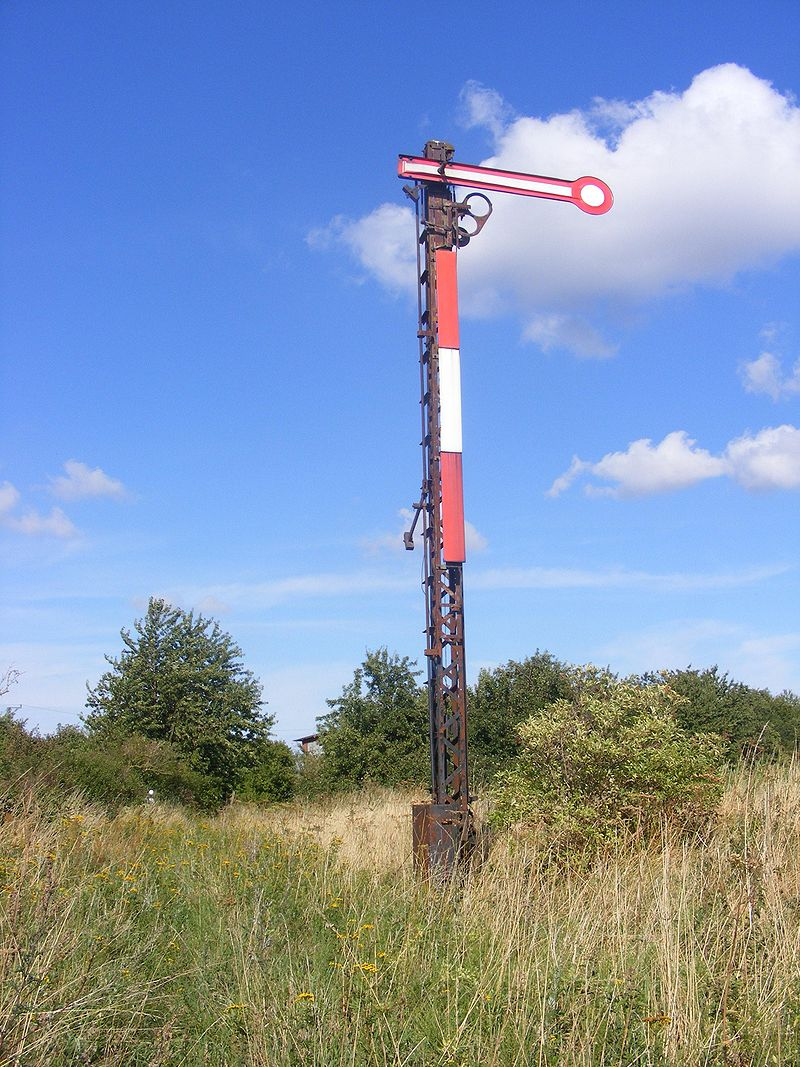
\includegraphics[scale=0.2]{../media/semaphor.jpg}
        \caption{Quelle: \href{https://de.wikipedia.org/wiki/Semaphor_(Informatik)}{Wikipedia}}
    \end{minipage}
\end{figure}

Im einfachsten Fall besteht sie einfach aus einem Wahrheitswert oder einer Ganzzahl, die den Zustand der Ressource beschreibt, einer Methode \q{Reservieren()}, die effektiv den Zugriff für alle anderen sperrt und \q{Freigeben()}, die die entsprechende Ressource wieder entsperrt. \\
Der Semaphor kann auch erweitert werden, sodass er als Warteschlange fungiert, z.B. könnte man den obigen Zähler erweitern und speichern, wie viele Prozesse gerade \q{warten}.
\textbf{Beispielbereiche für die Anwendung des Semaphor-Prinzips}
\begin{enumerate}
    \item \textbf{DBMS}
    \item \textbf{Druckerwarteschlangen}
    \item \textbf{Dateizugriff}
    \item \textbf{Verwaltung von Threads}: Auch bei Software an sich möchte man Parallelsierung nutzen, da es häufig Fälle gibt, bei denen ähnliche Dinge \q{gleichzeitig} ablaufen sollen bzw. berechnet werden, dazu werden \textbf{Threads} verwendet. 
\end{enumerate}
Der letzte Punkt bringt uns direkt zum nächsten Thema: 

\subsection{Parallele Prozesse in Java}

In den letzten zwei Jahrzehnten sind die Anforderungen an Prozessoren immens gewachsen, da immer größere Probleme mit Hilfe von Computern gelöst werden sollen, einige Beispiele:
\begin{enumerate}
    \item Klimasimulationen
    \item Strömungsmechanik
    \item Modellierung allgemein
    \item Animierte Filme
    \item Computerspiele
    \item Web-Suche (das Internet ist riesig! :)
\end{enumerate}
\newpage
Obwohl der Film schon etwas älter ist, sind die Zahlen bei Baymax beeindruckend:
\begin{center}
    
\includegraphics[scale=1.1]{../media/baymax.png} \\
    \textit{Quelle}: \href{https://disney.fandom.com/wiki/Big_Hero_6/Gallery}{disney.fandom} 
\end{center}
Der Film wurde auf einem Cluster von 4.600 Rechnern mit insgesamt 55.000 Kernen erstellt mit einer kumulierten Rechenzeit von 200 Millionen Stunden. Das entspricht einer Rechenzeit von etwa 83 Stunden pro Frame! \\
Ohne Parallelisierung - d.h. ein einziger Kern rendert den kompletten Film - wäre solch ein Mammutprojekt nicht denkbar. \\
\textit{Hinweis:} Tatsächlich wäre eine reine Parallelisierung immer noch nicht ausreichend, um die gigantischen Anforderungen des Rendering abzufangen, die größten Verbesserungen kommen durch die Verwendung intelligenter Algorithmen, die Parallelisierung schadet aber natürlich nicht. \\

An dieser Stelle könnte man einen langen Exkurs einfügen, wie wichtig Parallelität in den meisten Bereichen der Technik inzwischen ist, dafür haben wir hier aber keine Zeit. \vspace{5mm} \\

\textbf{Umsetzung in Java}

Die Umsetzung in Java wird uns noch in der zwölften Klasse ausführlich beschäftigen, hier ein kleiner Vorgeschmack: 
\begin{minted}{java}
public class Threading{
    public static void main(String[] args) {
        // Wir erzeugen die Threads und geben ihnen eine Aufgabe
        Thread t1 = new Thread(new Task());
        Thread t2 = new Thread(new Task());
        
        // Wir starten die Threads.
        t1.start();
        t2.start();
        
        // Wir warten darauf, dass beide Threads fertig sind.
        try {
            t1.join();
            t2.joint();
        } catch (InterruptedException e) {
            e.printStackTrace();
        }
        System.out.println("Task finished");
    }
    }

    class Task implements Runnable {
    @Override
    public void run() {
        // Irgendeine Aufgabe wird ausgeführt. 
        System.out.println("Task executed by " + Thread.currentThread().getName());
    }
}
\end{minted}
Die Verwendung von Threads ist in Java grundsätzlich nicht schwer, da bereits eine vorgebaute Klasse \textbf{Thread} existiert, die dem entsprechenden Betriebssystem mitteilt, dass möglichst ein zweiter Kern genutzt werden soll. \\
Natürlich ergibt sich hier aber ein analoges Problem zum vorigen Kapitel, wenn die Aufgabe, die jeder Thread ausführt auf gemeinsame Ressourcen zugreifen muss, so kann es zu den bereits besprochenen Problemen kommen. \\
Wie Java diese Probleme löst ist Stoff der 12. Klasse. 

\end{document}